\documentclass[a4paper,10pt]{article}
\usepackage[utf8]{inputenc}
\usepackage{graphicx}
\usepackage{float}
\usepackage[parfill]{parskip}
\usepackage{listings}

\begin{document}

\section{Conceptual Model}
\begin{figure}[H]
\centering
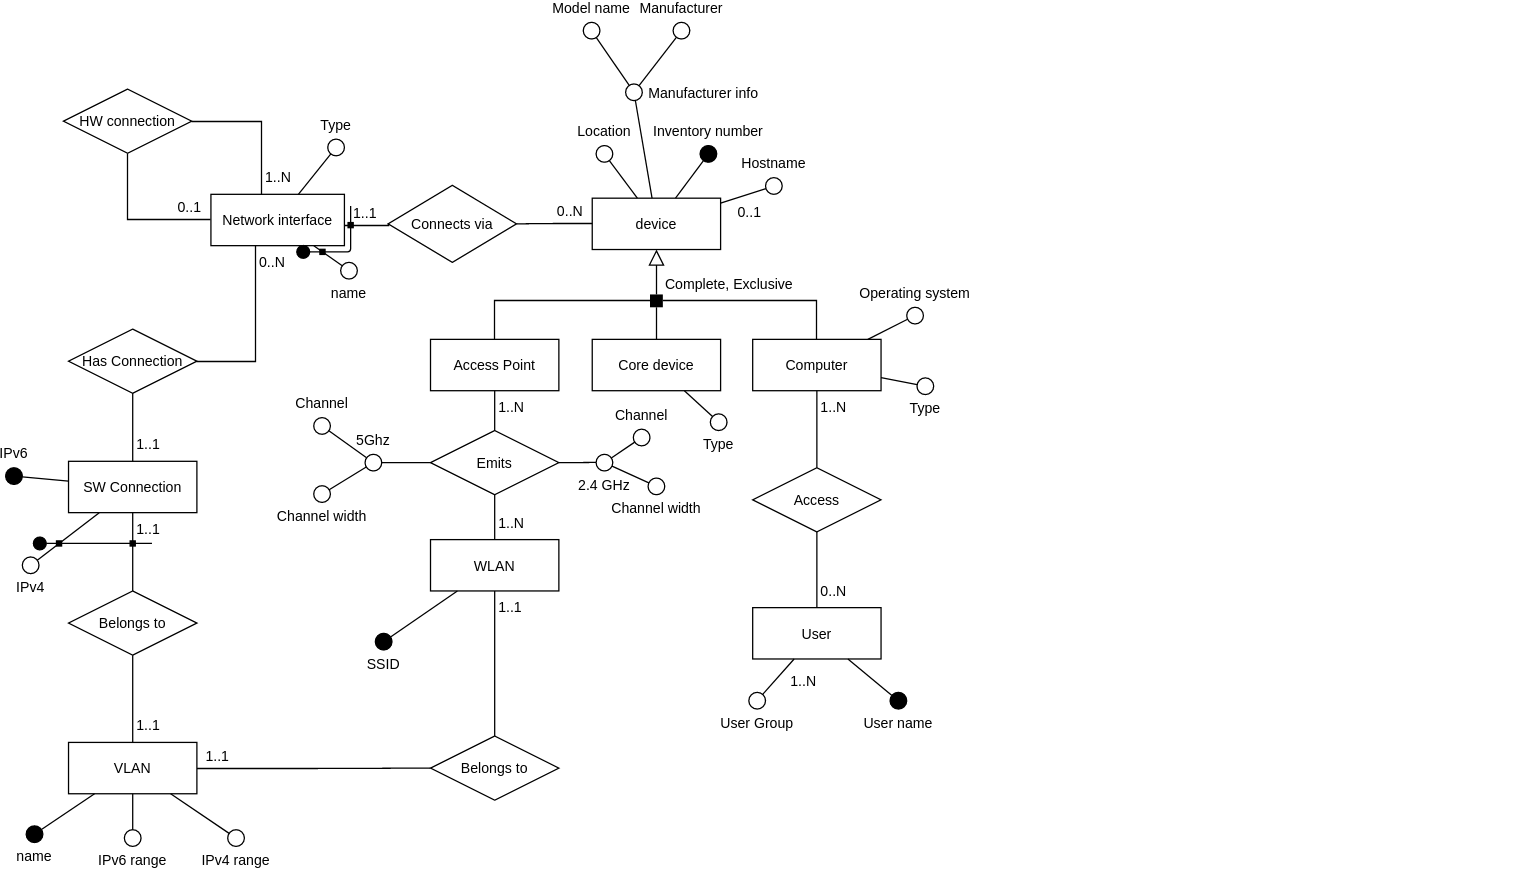
\includegraphics[width=15cm]{er.png}
\caption{ER diagram}
\end{figure}

\section{Relational Model}
Device(\underline{invNo}, location, hostname, modelName, manufacturer)

Computer(\underline{device}, os, type)\\
\hspace*{1em}FK: (device) \(\subseteq\) Device(invNo)

User(\underline{username})

UserGroup(\underline{user, name})\\
\hspace*{1em}FK: (user) \(\subseteq\) User(username)

Access(\underline{computer, user})\\
\hspace*{1em}FK: (computer) \(\subseteq\) Computer(device)\\
\hspace*{1em}FK: (user) \(\subseteq\) User(username)

CoreDevice(\underline{device}, type)\\
\hspace*{1em}FK: (device) \(\subseteq\) Device(invNo)

AccessPoint(\underline{device})\\
\hspace*{1em}FK: (device) \(\subseteq\) Device(invNo)

VLAN(\underline{name}, IPv4Range, IPv6Range)

WLAN(\underline{ssid}, vlan)\\
\hspace*{1em}FK: (vlan) \(\subseteq\) VLAN(name)

APEmits(\underline{ap, network}, channel5Ghz, width5Ghz, channel2Ghz, width2Ghz)\\
\hspace*{1em}FK: (ap) \(\subseteq\) AccessPoint(device)\\
\hspace*{1em}FK: (network) \(\subseteq\) WLAN(ssid)

Interface(\underline{device, name}, type)\\
\hspace*{1em}FK: (device) \(\subseteq\) Device(invNo)

\textit{Source can have multiple targets, but target is connected only to one}\\
source HWConnection(\underline{sourceName, sourceDevice, targetName, targetDevice})\\
\hspace*{1em}FK: (sourceName, sourceDevice) \(\subseteq\) Interface(name, device)\\
\hspace*{1em}FK: (targetName, targetDevice) \(\subseteq\) Interface(name, device)

SWConnection(\underline{ipv6}, \underline{ipv4, vlan}, interface, device)\\
\hspace*{1em}FK: (interface, device) \(\subseteq\) Interface(name, device)\\
\hspace*{1em}FK: (vlan) \(\subseteq\) VLAN(name)

\section{SQL}
\begin{figure}[H]
\centering
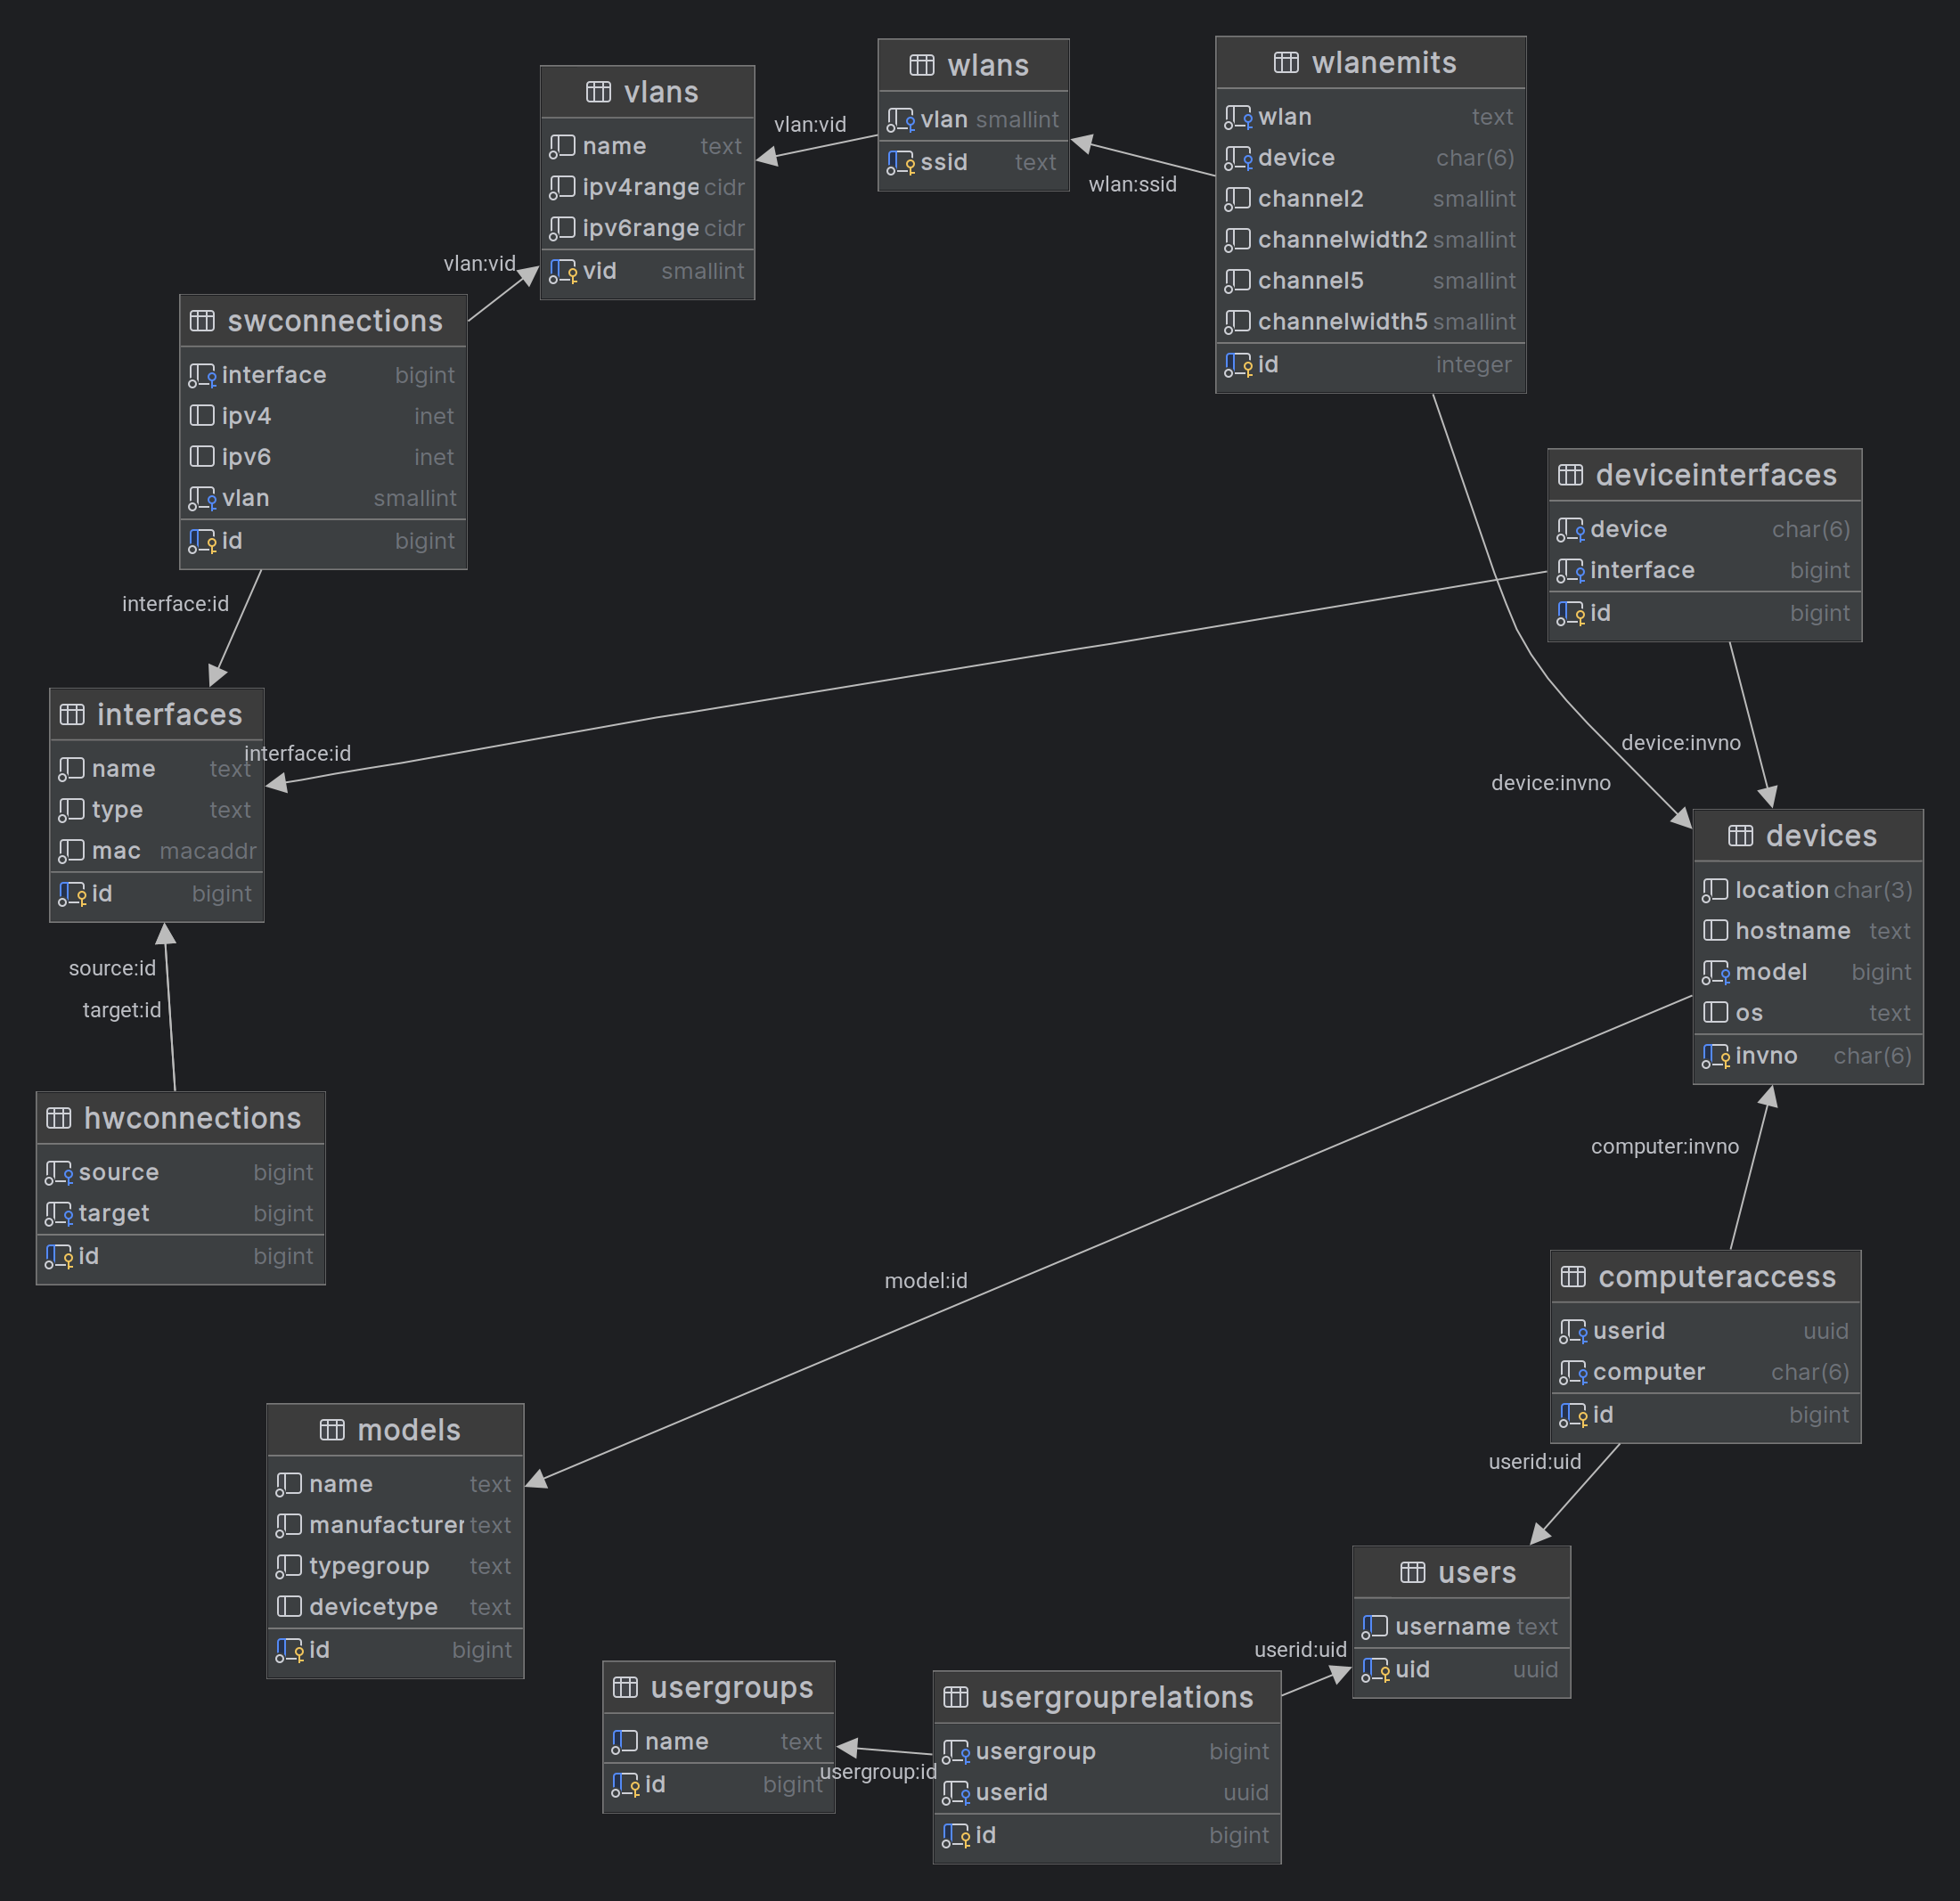
\includegraphics[width=15cm]{db.png}
\caption{DB diagram}
\end{figure}
\subsection{Creation}

\begin{lstlisting}[language=SQL]
CREATE TABLE models
(
    id           BIGSERIAL,
    name         TEXT NOT NULL,
    manufacturer TEXT NOT NULL,
    typeGroup    TEXT NOT NULL DEFAULT 'computer',
    deviceType   TEXT,
    CONSTRAINT Model_pk PRIMARY KEY ("id"),
    CONSTRAINT Model_typeGroup_values CHECK (
        typeGroup IN ('computer', 'ap', 'core')
        )
);

CREATE TABLE devices
(
    invNo    CHAR(6),
    location CHAR(3)   NOT NULL,
    hostname TEXT,
    model    BIGSERIAL NOT NULL,
    os       TEXT,
    CONSTRAINT Device_pk PRIMARY KEY (invNo),
    CONSTRAINT Device_model FOREIGN KEY (model)
        REFERENCES models (id) ON DELETE SET NULL
);

CREATE TABLE vlans
(
    vid       SMALLINT,
    name      TEXT NOT NULL,
    ipv4range CIDR NOT NULL,
    ipv6range CIDR NOT NULL,
    CONSTRAINT Vlan_pk PRIMARY KEY (vid),
    CONSTRAINT Vlan_vid CHECK ( (vid > 0) AND (vid < 4095) )
);

CREATE TABLE wlans
(
    ssid TEXT,
    vlan SMALLINT NOT NULL,
    CONSTRAINT Wlan_pk PRIMARY KEY (ssid),
    CONSTRAINT Wlan_fk_ssid FOREIGN KEY (vlan)
        REFERENCES vlans (vid) ON DELETE SET NULL
);

CREATE TABLE wlanEmits
(
    id            SERIAL,
    wlan          TEXT     NOT NULL,
    device        CHAR(6)  NOT NULL,
    channel2      SMALLINT NOT NULL,
    channelWidth2 SMALLINT NOT NULL,
    channel5      SMALLINT NOT NULL,
    channelWidth5 SMALLINT NOT NULL,
    CONSTRAINT WlanEmits_pk PRIMARY KEY (id),
    CONSTRAINT WlanEmits_wlan FOREIGN KEY (wlan)
        REFERENCES wlans (ssid) ON DELETE CASCADE,
    CONSTRAINT WlanEmits_device FOREIGN KEY (device)
        REFERENCES devices (invNo) ON DELETE CASCADE,
    CONSTRAINT WlanEmits_channel2 CHECK (
            channel2 IN (
                         1, 2, 3, 4, 5, 6, 7, 8, 9, 10, 11, 12, 13
            )
        ),
    CONSTRAINT WlanEmits_chanelWidth2 CHECK (
        channelWidth2 IN (20, 40)
        ),
    CONSTRAINT WlanEmits_channel5 CHECK (
            channel5 IN (
                         32, 34, 36, 38, 40, 42, 44, 46,
                         48, 50, 52, 54, 56, 58, 60, 62,
                         64, 68, 96, 100, 102, 104, 106,
                         108, 110, 112, 114, 116, 118,
                         120, 122, 124, 126, 128, 132,
                         134, 136, 138, 140, 142, 144,
                         149, 151, 153, 155, 157, 159,
                         161, 165, 167, 169, 171,
                         173
            )
        ),
    CONSTRAINT WlanEmits_channelWidth5 CHECK (
        channelWidth5 IN (20, 40, 80)
        )
);

CREATE TABLE interfaces
(
    id   BIGSERIAL,
    name TEXT    NOT NULL,
    type TEXT    NOT NULL DEFAULT 'ethernet',
    mac  MACADDR NOT NULL,
    CONSTRAINT Interface_pk PRIMARY KEY (id),
    CONSTRAINT Interface_type CHECK (
            type IN ('ethernet', 'radio', 'sfp+', 'qsfp+')
        )
);

CREATE TABLE swConnections
(
    id        BIGSERIAL,
    interface BIGSERIAL NOT NULL,
    ipv4      INET,
    ipv6      INET,
    vlan      SMALLINT  NOT NULL,
    CONSTRAINT SwConnection_pk PRIMARY KEY (id),
    CONSTRAINT SwConnection_vlan FOREIGN KEY (vlan)
        REFERENCES vlans (vid) ON DELETE CASCADE,
    CONSTRAINT SwConnection_interface FOREIGN KEY (interface)
        REFERENCES interfaces (id) ON DELETE CASCADE,
    CONSTRAINT SwConnection_ip CHECK ( (ipv4 IS NOT NULL) OR
                                       (ipv6 IS NOT NULL) )
);

CREATE TABLE hwConnections
(
    id     BIGSERIAL,
    source BIGSERIAL NOT NULL,
    target BIGSERIAL NOT NULL,
    CONSTRAINT HwConnection_pk PRIMARY KEY (id),
    CONSTRAINT HwConnection_source FOREIGN KEY (source)
        REFERENCES interfaces (id) ON DELETE CASCADE,
    CONSTRAINT HwConnection_target FOREIGN KEY (target)
        REFERENCES interfaces (id) ON DELETE CASCADE
);

CREATE TABLE deviceInterfaces
(
    id        BIGSERIAL,
    device    CHAR(6)   NOT NULL,
    interface BIGSERIAL NOT NULL,
    CONSTRAINT DeviceInterfaces_pk PRIMARY KEY (id),
    CONSTRAINT DeviceInterfaces_device FOREIGN KEY (device)
        REFERENCES devices (invNo) ON DELETE CASCADE,
    CONSTRAINT DeviceInterfaces_interface FOREIGN KEY (interface)
        REFERENCES interfaces (id) ON DELETE CASCADE
);

CREATE TABLE users
(
    uid      UUID,
    username TEXT NOT NULL UNIQUE,
    CONSTRAINT User_pk PRIMARY KEY (uid)
);

CREATE TABLE computerAccess
(
    id       BIGSERIAL,
    userId   UUID    NOT NULL,
    computer CHAR(6) NOT NULL,
    CONSTRAINT ComputerAccess_pk PRIMARY KEY (id),
    CONSTRAINT ComputerAccess_userId FOREIGN KEY (userId)
        REFERENCES users (uid) ON DELETE CASCADE,
    CONSTRAINT ComputerAccess_computer FOREIGN KEY ("computer")
        REFERENCES devices (invNo) ON DELETE CASCADE
);

CREATE TABLE userGroups
(
    id   BIGSERIAL,
    name TEXT NOT NULL UNIQUE,
    CONSTRAINT UserGroup_pk PRIMARY KEY (id)
);

CREATE TABLE userGroupRelations
(
    id        BIGSERIAL,
    userGroup BIGSERIAL NOT NULL,
    userId    UUID      NOT NULL,
    CONSTRAINT UserGroupRelations_pk PRIMARY KEY (id),
    CONSTRAINT UserGroupRelations_userGroup FOREIGN KEY (userGroup)
        REFERENCES userGroups (id) ON DELETE CASCADE,
    CONSTRAINT UserGroupRelations_userId FOREIGN KEY (userId)
        REFERENCES users (uid) ON DELETE CASCADE
);

\end{lstlisting}

\subsection{Selection}
\begin{lstlisting}[language=SQL]
SELECT *
FROM swconnections
         RIGHT OUTER JOIN vlans
                          ON (swconnections.ipv4 <<= vlans.ipv4range);

SELECT *
FROM devices
         JOIN models
              ON (devices.model = models.id);

SELECT *
FROM swconnections
WHERE ipv4 = '192.168.32.1';

SELECT COUNT(DISTINCT channel2) AS channels2,
       count(DISTINCT channel5) AS channels5
FROM wlanemits;

SELECT *
FROM models
ORDER BY manufacturer;

SELECT *, MASKLEN(ipv6)
FROM swconnections
WHERE (MASKLEN( ipv6 ) > (
    SELECT AVG(MASKLEN( ipv6 ) ) FROM swconnections )
) ;
\end{lstlisting}


\end{document}
